\section{Experiments}
\label{sec:experiments}

\subsection{Data, Protocol, and Comparisons}
We use BCI Competition IV-2b \cite{tangermann2012bciciv}, which contains three EEG and three EOG channels
sampled at 250 Hz. All nine participants are development participants. For each
participant and each of three frozen same-session units, early EEG+EOG forms
support and later EEG+EOG forms query; support and query time ranges do not
overlap. Table~\ref{tab:protocol} summarizes the evidence unit and information
boundary. Query EOG is an explicit deployment input.

\begin{table}[t]
\caption{Frozen same-session development protocol.}
\label{tab:protocol}
\centering
\begin{tabular}{ll}
\toprule
Item & Frozen value\\
\midrule
Participants & 9 development participants\\
Scientific unit & Participant ($n=9$)\\
Within-participant units & 3 same-session units\\
Support & Early synchronized EEG+EOG\\
Query input & Later EEG+EOG\\
Model seeds & 20260808, 20260810, 20260811\\
Population training & 7 subjects; recipient and cyclic donor held out\\
Primary sampler & DDIM25, $K=8$ arithmetic mean\\
Evaluator-only & paired target; natural labels and outcome fields\\
\bottomrule
\end{tabular}
\end{table}

Paired rows combine real low-EOG EEG carriers and real EOG-derived ocular
components from nonoverlapping time ranges. We report RRMSE, waveform
correlation, $\Delta$SNR, and 1--45 Hz paired spectral utility. These targets
support controlled reconstruction comparisons, not a claim of natural clean
ground truth. Natural motor-imagery EEG provides EOG attenuation,
low-artifact preservation, MI-band PSD distortion, covariance distortion,
ERD/ERS preservation, and a frozen downstream MI readout.

The core methods are RAW; LINEAR-MATCH from Eq.~\eqref{eq:linear_anchor};
DET-MATCH from Eq.~\eqref{eq:det_residual}; and the same fixed diffusion model
under population, matched, and cyclic unseen-wrong operators. DIFF-TEMPORAL-
SHUFFLED and compatible seen-donor operators are secondary controls. The primary
subject effects are
\begin{align}
 U_P&=R(\mathrm{DIFF\mbox{-}POP})-R(\mathrm{DIFF\mbox{-}MATCH}),\\
 U_W&=R(\mathrm{DIFF\mbox{-}WRONG})-R(\mathrm{DIFF\mbox{-}MATCH}),
\end{align}
where $R$ is participant-level paired RRMSE and positive values favor matching.

\subsection{Aggregation and Statistical Scope}
Windows are aggregated within each same-session unit, units within participant,
and then the three training seeds within participant. Thus $n=9$; the 27
participant--seed comparisons are stability measurements, not independent
scientific samples. We report the exact one-sided sign-flip test aligned with
the directional hypothesis and a two-sided sensitivity test. With 9/9 signs in
the same direction, these are $p=0.001953$ and $p=0.003906$, respectively.
Participant bootstrap intervals use 20,000 resamples and are descriptive because
the cohort was used throughout development.

For interpretation only, we define
\begin{equation}
 I_P=[R(\mathrm{DET\mbox{-}POP})-R(\mathrm{DET\mbox{-}MATCH})]
 -[R(\mathrm{DIFF\mbox{-}POP})-R(\mathrm{DIFF\mbox{-}MATCH})].
\end{equation}
A positive $I_P$ means the deterministic subject benefit is larger; it is not
evidence of diffusion-specific synergy. No interaction sign is a study gate.

\subsection{Subject-Conditioning Results}
Table~\ref{tab:main} gives three-seed method means. DIFF-MATCH improves RRMSE
over DIFF-POP by $U_P=0.03473$ (median $0.03338$; descriptive 95\% interval
$[0.02899,0.04079]$) and over the cyclic unseen-WRONG by $U_W=0.04836$
(median $0.03862$; $[0.02987,0.07220]$). Both effects are positive for all nine
participants (Fig.~\ref{fig:effects}).

\begin{table*}[t]
\caption{Three-seed development means. Lower RRMSE is better; correlation,
$\Delta$SNR, attenuation, and preservation are higher-is-better.}
\label{tab:main}
\centering
\begin{tabular}{lrrrrrr}
\toprule
Method & RRMSE $\downarrow$ & Corr. $\uparrow$ & $\Delta$SNR $\uparrow$ & EOG attn. $\uparrow$ & Preserv. $\uparrow$ & Cov. dist. $\downarrow$\\
\midrule
RAW & 0.48851 & 0.89717 & 0.0000 & 0.0000 & 1.0000 & 0.0000\\
LINEAR-MATCH & \textbf{0.08760} & 0.99304 & 18.0654 & 0.0973 & 0.8123 & 0.0909\\
DET-MATCH & 0.11225 & \textbf{0.99319} & 12.5072 & 0.1039 & 0.7979 & 0.1248\\
DIFF-POP & 0.14823 & 0.98818 & 9.9214 & 0.0987 & 0.7920 & 0.1241\\
DIFF-MATCH & 0.11350 & 0.99289 & 12.3898 & \textbf{0.1043} & 0.7982 & 0.1237\\
DIFF-WRONG & 0.16186 & 0.98415 & 9.6218 & 0.0987 & 0.7926 & 0.1237\\
\bottomrule
\end{tabular}
\end{table*}

\begin{figure*}[t]
\centering

\includegraphics[width=0.92\textwidth]{figures/participant_effects.pdf}
\caption{Participant-level subject effects after averaging the three training
seeds. Positive values indicate lower RRMSE for DIFF-MATCH. Every participant
is positive for both the population ($U_P$) and frozen cyclic unseen-WRONG
($U_W$) comparison. Intervals are descriptive participant bootstrap intervals.}
\label{fig:effects}
\Description{Two participant point plots show positive effects for each of nine
participants and positive mean effects for population and wrong controls.}
\end{figure*}

The per-seed mean $U_P$ values are $0.03654$, $0.03465$, and $0.03299$; mean
$U_W$ values are $0.04667$, $0.04779$, and $0.05062$. Each seed has 9/9 positive
participants for both comparisons. Figure~\ref{fig:seed_heatmap} shows that the
direction is not created by seed averaging.

\begin{figure}[t]
\centering

\includegraphics[width=\linewidth]{figures/seed_effect_heatmap.pdf}
\caption{Participant-by-seed effects. Training seeds are stability repeats on
the same development cohort and are not independent samples.}
\label{fig:seed_heatmap}
\Description{A heatmap shows positive population and wrong effects for every
participant and all three training seeds.}
\end{figure}

The primary specificity control is the frozen cyclic unseen-WRONG. Each fold
has one truly unseen donor. All seven compatible population-training donors
were also evaluated separately as a sensitivity analysis: the recipient--seed
mean utility is $0.03976$ (27/27 positive). The single unseen donor sensitivity
is $0.04876$ (27/27 positive), but this is the same donor role as the primary
cyclic control and is not a multi-unseen-donor replication.

\subsection{Natural-Signal Proxies and Exceptions}
Mean natural-signal proxy criteria were met, with disclosed participant-level
exceptions. DIFF-MATCH has mean EOG attenuation $0.1043$, preservation $0.7982$,
covariance distortion $0.1237$, and MI-band PSD distortion $0.0719$. Relative
MI kappa versus DIFF-POP is $+0.0032$. At the participant level, EOG attenuation
is nonpositive for 0/9, preservation is below $0.78$ for 1/9, covariance
distortion exceeds $0.15$ for 2/9, and the MI-kappa margin is below $-0.02$ for
0/9. Accordingly, we do not claim uniform safety.

\begin{figure*}[t]
\centering

\includegraphics[width=0.96\textwidth]{figures/waveform_psd.pdf}
\caption{Pre-frozen example: participant 1, first same-session unit, first paired
window, first EEG channel, seed 20260808. The rule was fixed by indices rather
than by outcome. PSD uses the valid first 500 samples.}
\label{fig:waveform}
\Description{Waveforms and PSDs compare raw, linear match, diffusion population,
diffusion match, diffusion wrong, and the paired clean target for a fixed case.}
\end{figure*}

Figure~\ref{fig:safety} places participant-level EOG attenuation beside
preservation and identifies the frozen safety reversals. It is a proxy analysis,
not a claim that all neural activity is preserved.

\begin{figure}[t]
\centering
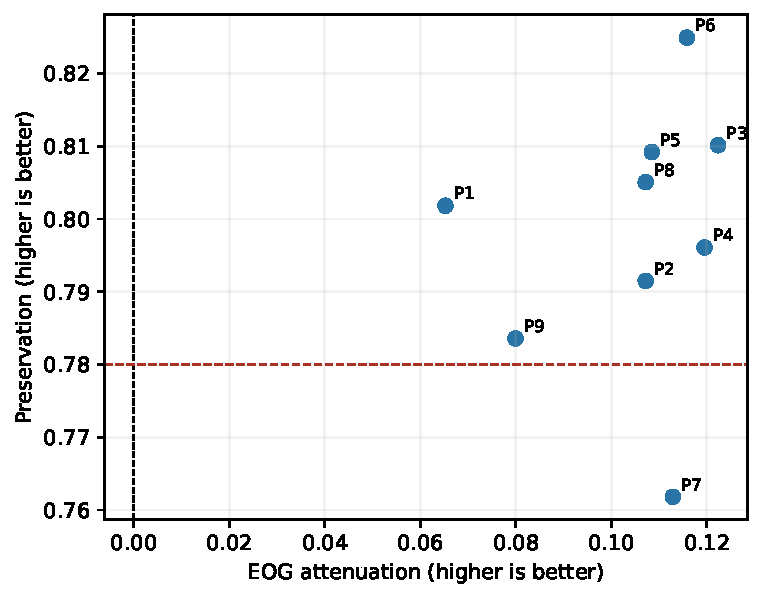
\includegraphics[width=\linewidth]{figures/attenuation_preservation.pdf}
\caption{Participant-level natural EEG attenuation--preservation trade-off for
DIFF-MATCH. Dashed lines mark zero attenuation and preservation 0.78.}
\label{fig:safety}
\Description{All participants have positive EOG attenuation; one lies below the
preservation reference line.}
\end{figure}

\subsection{Comparison Boundary and Compute}
The subject effect must not be conflated with diffusion superiority.
DIFF-MATCH RRMSE ($0.11350$) is slightly worse than DET-MATCH ($0.11225$) and
worse than LINEAR-MATCH ($0.08760$). Thus diffusion-over-deterministic and
diffusion-over-linear are \emph{not supported}. The mean $I_P$ is also positive
and small across seeds, indicating that the deterministic subject benefit is
slightly larger rather than showing diffusion-specific synergy.

DDIM25 with $K=8$ uses 200 network calls, $0.0166$ seconds per window on the
recorded GPU runs, and a peak allocated memory of 177 MB. These resource values
locate the frozen implementation and are not scientific gates.

\subsection{Evidence Boundary}
This is three-seed stability on the same nine-participant development cohort,
not evaluation on an independent cohort or confirmation. The population model
uses seven training subjects because the recipient and cyclic donor are held
out. The result establishes a matched-operator effect inside one EOG-guided
pipeline; it does not establish EEG-only denoising, general artifact removal,
benchmark leadership, or a diffusion-specific personalization effect.
